%====================
% BUILD: xelatex cv.tex
%====================
\documentclass[a4paper]{cv}

\usepackage{enumitem}
\usepackage{multicol}

\graphicspath{{image/}}

\begin{document}

%====================
% HEADER
%====================
\header{radovan}{kuka}{Web Developer \& Front-end Expert}

%====================
% SIDE BLOCK
%====================

\begin{aside}
	% Photo
	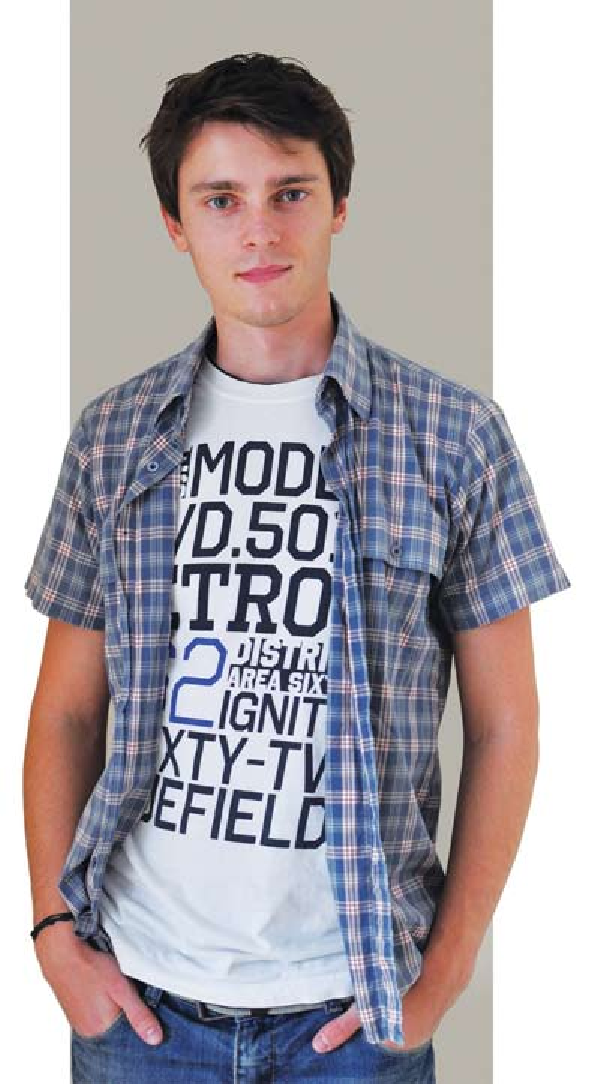
\includegraphics[scale=0.48]{photo.pdf}
	\about{I am a software engineer with strong analytical and logical thinking, highly motivated by challenges and interesting projects. I am focused on web design and modern web technologies, especially HTML5 and JavaScript. I am a keen learner always seeking to improve my skills and keeping my knowledge up to date.}
	% webpage
	\webpage{www.radovankuka.com}
	% Email
	\email{kuka.radovan@gmail.com}
	% Cellphone
	\phone{(+421) 907 336 220}
	% Address
	\address{Banícka 21}{902 01 Pezinok}
	% Links
	\section{\vspace{5mm}\linkedIn{http://www.linkedin.com/in/radovankuka}   \github{https://github.com/kuka-radovan}   \twitter{https://twitter.com/radovan_kuka}   \facebook{https://www.facebook.com/kuka.radovan}}
\end{aside}

%====================
% EXPERIENCE
%====================
\section{experience}
\begin{entrylist}
	\entry
		{Senior Front-End Developer (Freelance)}
		{04/2017 - Present}
		{\emph{IN2CORE}\\
		I was hired to kickoff front-end part of cloud based solution of existed software tool for video assist professionals named QTAKE.}
	\entry
		{Front-End Team Lead}
		{06/2016 - 04/2017}
		{\emph{Pygmalios}\\
		I led highly motivated front-end team that is developing unique tool dedicated to customer behaviour analytics across retail segments.}
	\entry
		{Senior Front-End Developer}
%		{04/2015 - 06/2016}
		{05/2014 - 06/2016}
		{\emph{Piano Media}\\
		Front-end developer of paywall system written in React.js using ES6 ({\emph{ES2015}}).}
%	\entry
%		{Team Leader \& Senior Front-End Developer}
%		{06/2014 - 04/2015}
%		{\emph{Datalan}\\
%		Leading front-end team, development and implementation in ExtJS framework (JavaScript) and providing expert consultations.}
	\entry
		{UI Designer \& Front-End Developer}
%		{03/2012 - 05/2014}
		{03/2012 - 05/2014}
		{\emph{Gratex International}\\
		Implementation of internal widgets in Dojo framework (JavaScript) and application screens for an international insurance company.}
%	\entry
%		{Java Developer}
%		{12/2010 - 03/2012}
%		{\emph{Vigour}\\
%		Front-end development of a banking system in Finantix framework (Java).}
\end{entrylist}

%====================
% EDUCATION
%====================
\section{education}
\begin{entrylist}
	\entry
		{Slovak University of Technology in Bratislava}
		{2011 - 2013}
		{\emph{Faculty of Informatics and Information Technologies (FIIT)}\\
		Master's degree \emph{(Software Engineering)}}
	\entry
		{Slovak University of Technology in Bratislava}
		{2007 - 2011}
		{\emph{Faculty of Informatics and Information Technologies (FIIT)}\\
		Bachelor's degree \emph{(Informatics)}}
	\entry
		{Gymnasium of Viliam Pauliny-Tóth in Martin}
		{2003 - 2007}
		{Graduated}
\end{entrylist}

%====================
% CERTIFICATES
%====================
\section{certificates}
\begin{entrylist}
	\entry
		{HTML5 Application Development Fundamentals}
		{06/2013}
		{\emph{Microsoft Technology Associate (MTA) \\ License: E310-5741}}
	\entry
		{MongoDB for Developers}
		{01/2014}
		{\emph{MongoDB, Inc.}}
\end{entrylist}

%====================
% EXPERTISE
%====================
\section{expertise}
\begin{multicols}{3}

	\centerline{\textbf{Development}}
	\begin{description}[style=multiline,leftmargin=1.8cm,font=\normalfont]
		\item[JavaScript] {\huge\color{red}$\circ\circ\circ\circ\circ$}
		\item[HTML5] {\huge\color{red}$\circ\circ\circ\circ\color{gray}\circ$}
		\item[CSS3] {\huge\color{red}$\circ\circ\circ\color{gray}\circ\circ$}
		%\item[C++] {\huge\color{red}$\circ\circ\circ\color{gray}\circ\circ$}
		%\item[Java] {\huge\color{red}$\circ\circ\circ\color{gray}\circ\circ$}
	\end{description}
	\vfill
	\columnbreak

	\centerline{\textbf{Frameworks \& Tools}}
	\begin{description}[style=multiline,leftmargin=1.8cm,font=\normalfont]
		\item[React] {\huge\color{red}$\circ\circ\circ\circ\color{gray}\circ$}
		\item[Redux] {\huge\color{red}$\circ\circ\circ\circ\color{gray}\circ$}
		%\item[JQuery] {\huge\color{red}$\circ\circ\color{gray}\circ\circ\circ$}
		%\item[OpenCV] {\huge\color{red}$\circ\circ\color{gray}\circ\circ\circ$}
		\item[Backbone] {\huge\color{red}$\circ\circ\circ\color{gray}\circ\circ$}
	\end{description}
	\vfill
	\columnbreak

	\centerline{\textbf{Languages}}
	\begin{description}[style=multiline,leftmargin=1.4cm,font=\normalfont]
		\item[Slovak] {\huge\color{red}$\circ\circ\circ\circ\circ$}
		\item[English] {\huge\color{red}$\circ\circ\circ\color{gray}\circ\circ$}
		\item[German] {\huge\color{red}$\circ\color{gray}\circ\circ\circ\circ$}
	\end{description}
	\vfill
	\columnbreak
\end{multicols}

%\section{social skills}
%	communicability, ambitiousness, flexibility, independence, ability to work in a team

\section{interests}
	graphic design, web development, development principles, design patterns, algorithms

%====================
% FOOTER
%====================
\footer{a}{b}{c}
\end{document}
